\documentclass{beamer}

\usepackage{pgf,pdfpages}

\mode<presentation>
{
    \usetheme{bunsen}
    \setbeamercovered{transparent}
    \setbeamertemplate{items}[circle]
}

% suppress navigation bar
\beamertemplatenavigationsymbolsempty

\usefonttheme[onlymath]{serif}
\setbeamerfont{frametitle}{size=\LARGE,series=\bfseries}

\defbeamertemplate{enumerate item}{mycircle}
{
    \begin{pgfpicture}{0ex}{0ex}{1.5ex}{0ex}
        \pgfbox[center,base]{\insertenumlabel.}
    \end{pgfpicture}
}
[action]
{\setbeamerfont{item projected}{size=\scriptsize}}
\setbeamertemplate{enumerate item}[mycircle]


\title{Sega Game Gear on a Chip}
\author{Max Thrun | Samir Silbak}
\institute{University of Cincinnati}
\date{Fall 2012}

\begin{document}

\maketitle

%
% background for the rest of the slides
%
\setbeamertemplate{background}
{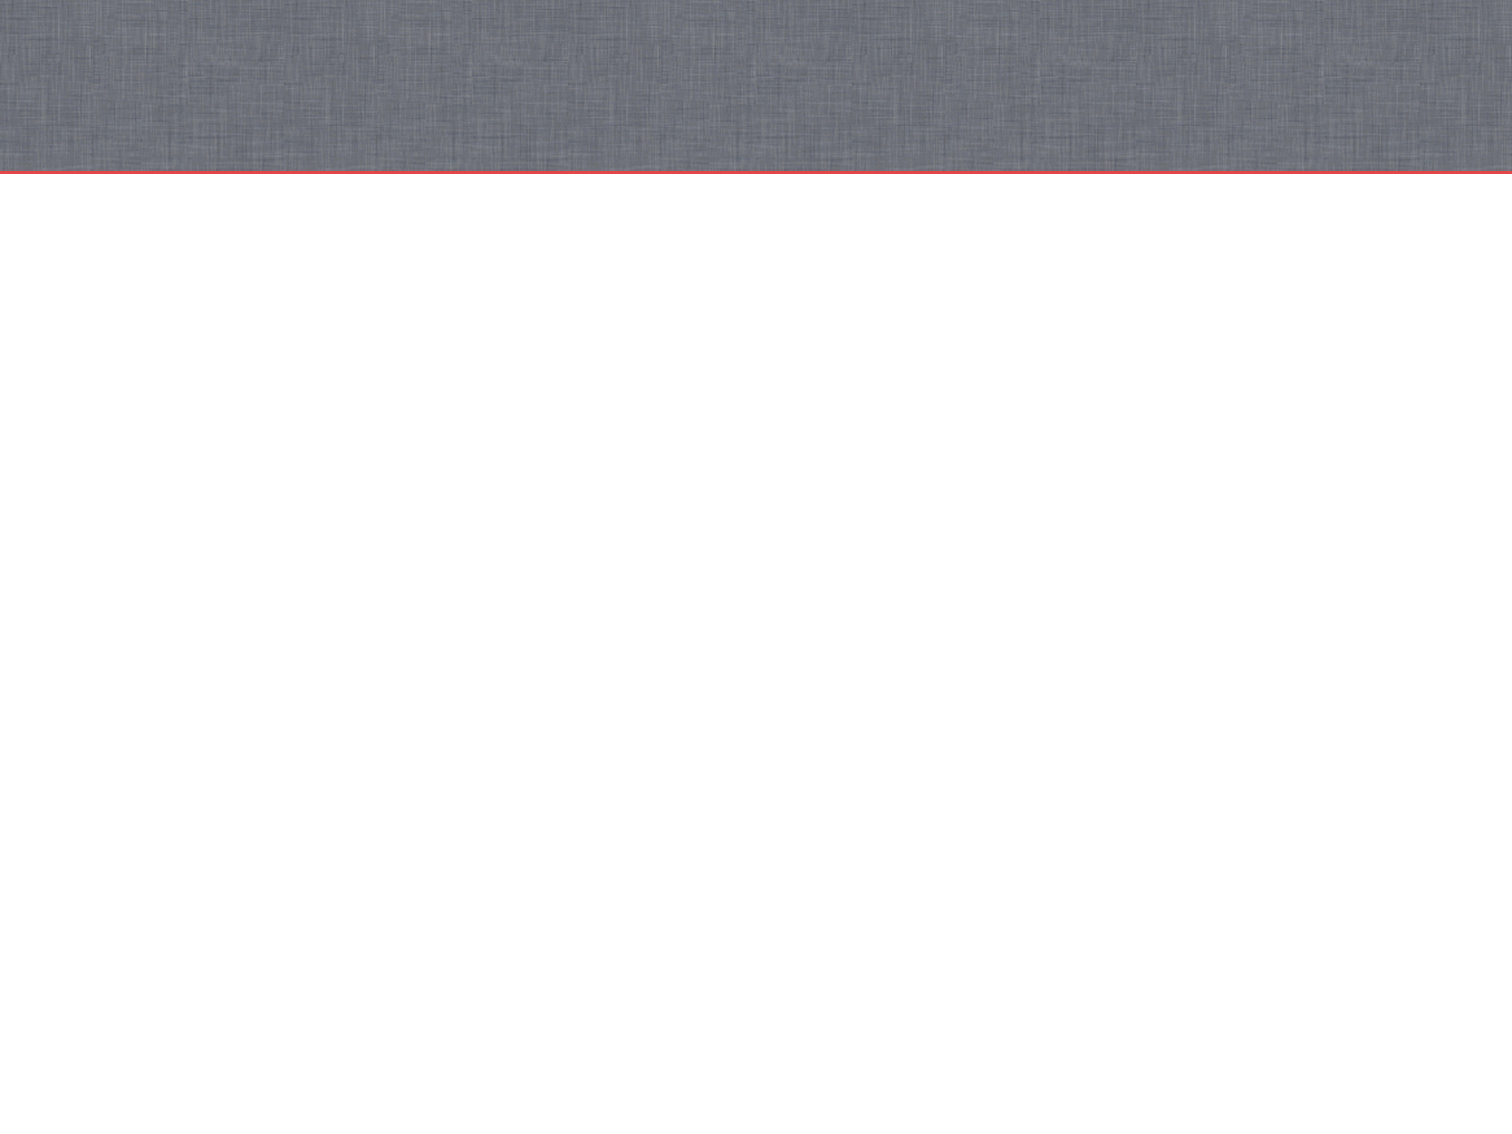
\includegraphics[width=\paperwidth,height=\paperheight]{slide_bg}}
\setbeamertemplate{footline}[bunsentheme]

\section{Introduction}
\begin{frame}
\frametitle{First slide}
some content here
\end{frame}

\section{Sega Game Gear}
\begin{frame}
    \frametitle{Sega Game Gear}
    \begin{center}
        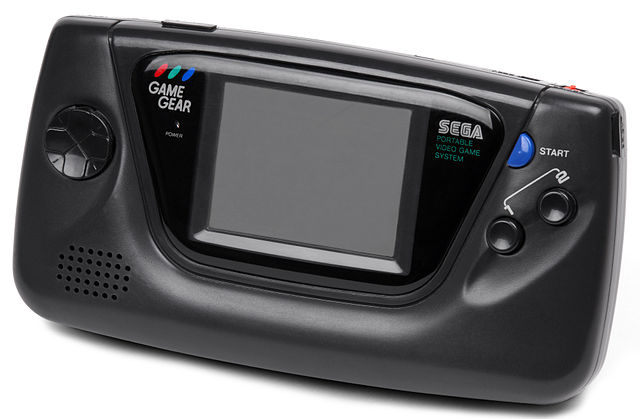
\includegraphics[width=0.6\textwidth]{gg.jpg}
    \end{center}
\end{frame}

\begin{frame}
    \frametitle{Sega Game Gear}

    \begin{columns}[c]
        \column{0.5\textwidth}
            \begin{itemize}
                \item Released April 1990
                \item Mobile version of the Sega Master System (functionally identical)
                \item Standard system architecture for the time (Z80 CPU, tri-state buses, etc...)
            \end{itemize}

        \column{0.5\textwidth}
            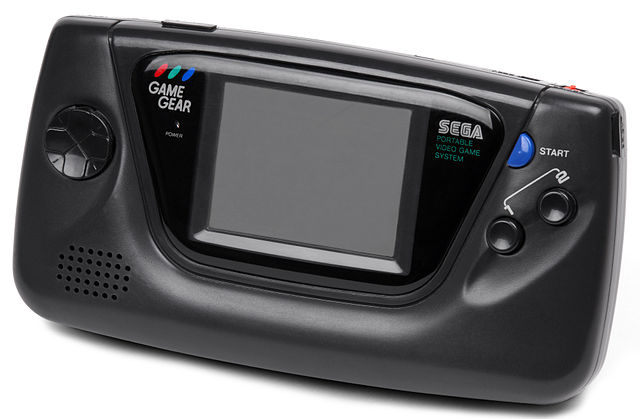
\includegraphics[width=\textwidth]{gg.jpg}
    \end{columns}
\end{frame}

\begin{frame}
    \frametitle{Sega Master System PCB}
    \begin{center}
        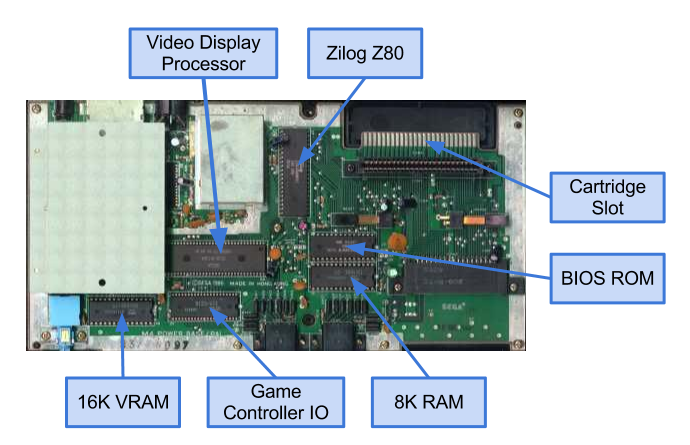
\includegraphics[width=\textwidth]{sms_pcb.png}
    \end{center}
\end{frame}

\section{System Diagrams}
\begin{frame}
    \frametitle{Black Box Diagram}
    \begin{center}
        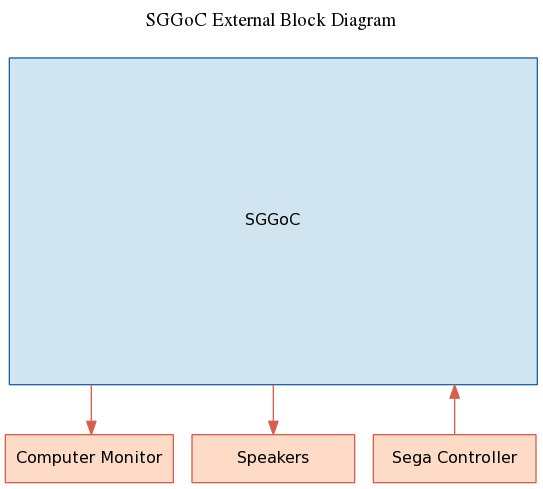
\includegraphics[width=\textwidth]{../block_diagrams/block_diagram_external.png}
    \end{center}
\end{frame}

\begin{frame}
    \frametitle{Transparent Box Diagram}
    \begin{center}
        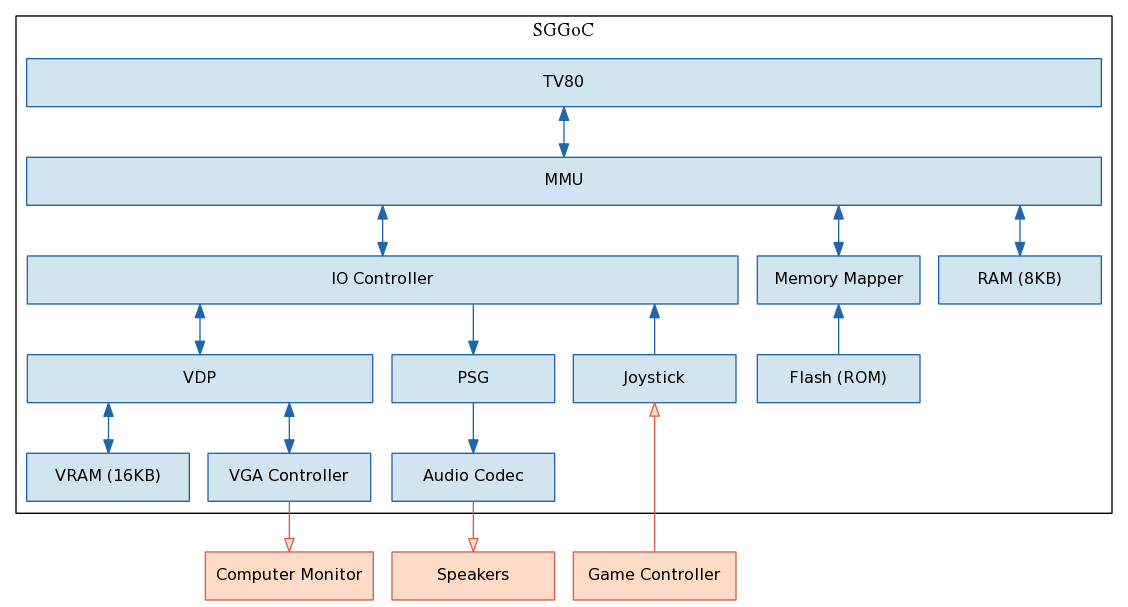
\includegraphics[width=\textwidth]{../block_diagrams/block_diagram_internal.png}
    \end{center}
\end{frame}

\section{Prototyping Platform}
\begin{frame}
    \frametitle{FPGA Development Board}
    \begin{center}
        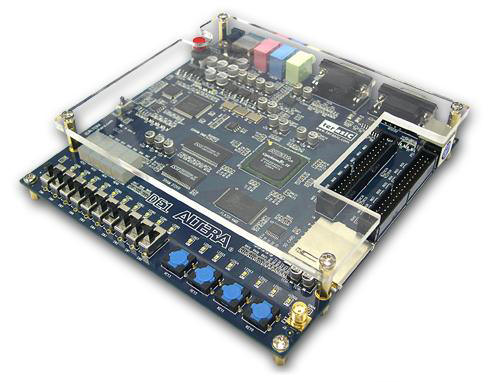
\includegraphics[height=0.7\textheight]{de1_angle.jpg}
    \end{center}
\end{frame}

\begin{frame}
    \frametitle{Altera DE1}

    \begin{columns}[c]
        \column{0.5\textwidth}
            \begin{itemize}
                \item Cyclone II EP2C20F484C7
                \item VGA, Audio, SD Card, 4 MB Flash
                \item Command line development environment
                \item Extremely good documentation
            \end{itemize}

        \column{0.5\textwidth}
            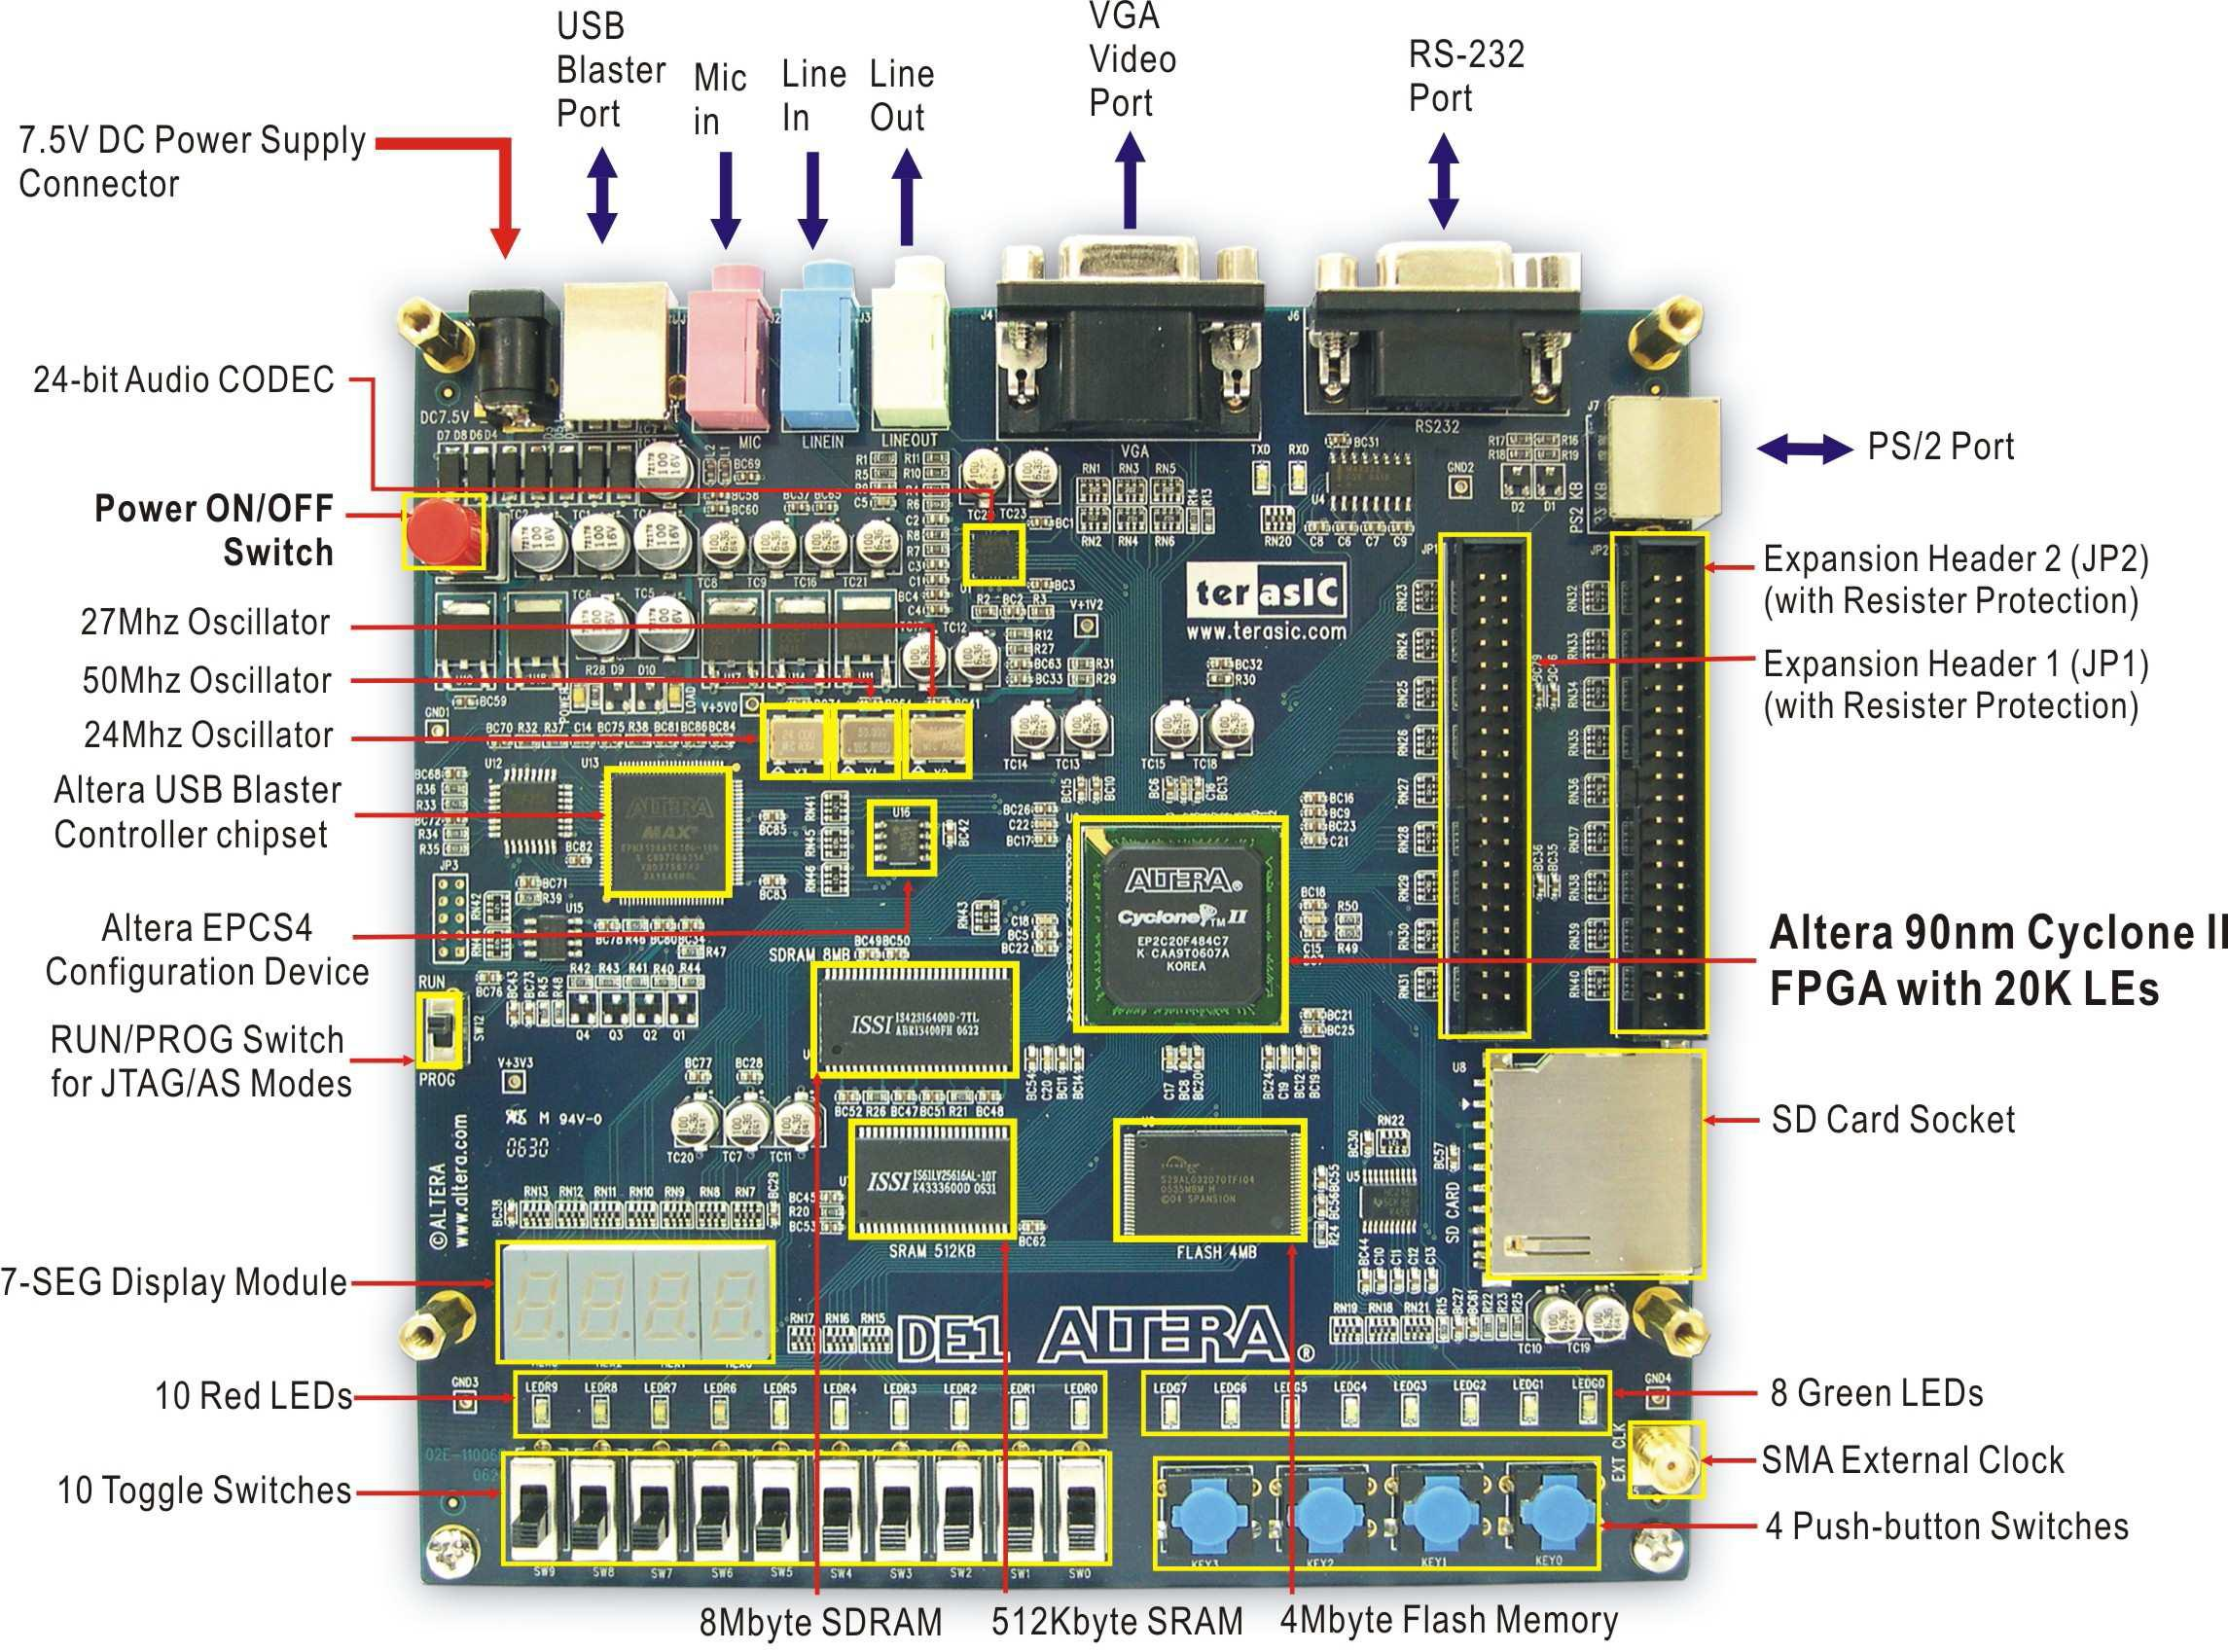
\includegraphics[width=\textwidth]{de1.jpg}
    \end{columns}
\end{frame}

\section{Game ROMs}
\begin{frame}
    \frametitle{Game Cartridge}

    \begin{columns}[c]
        \column{0.5\textwidth}
            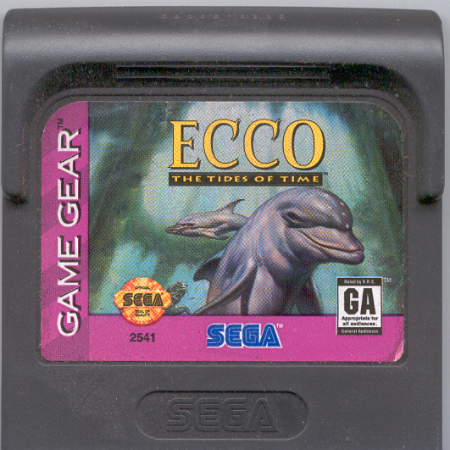
\includegraphics[width=\textwidth]{../design/gg_cart.png}
        \column{0.5\textwidth}
            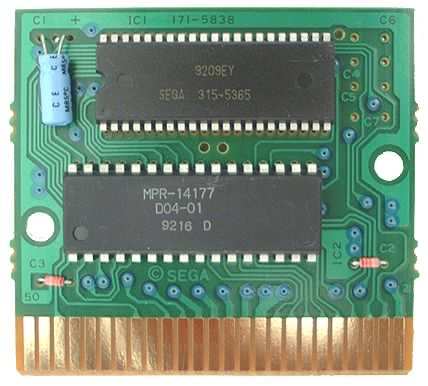
\includegraphics[width=\textwidth]{../design/gg_cart_pcb.png}
    \end{columns}
\end{frame}

\begin{frame}
    \frametitle{Game Cartridge}

    \begin{columns}[c]
        \column{0.5\textwidth}
            Each game cartridge made up of at least two components:
            \begin{itemize}
                \item<2->Game data ROM
                \item<3->Memory Mapper
            \end{itemize}
            \includegraphics<4->[width=\textwidth]{../design/mapper.png}

        \column{0.5\textwidth}
            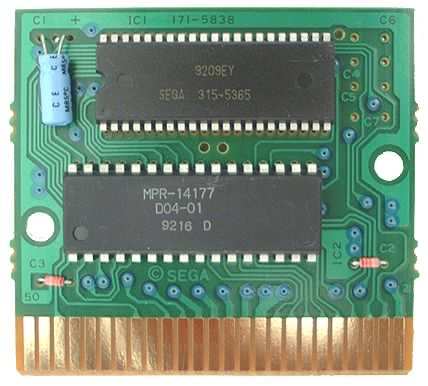
\includegraphics[width=\textwidth]{../design/gg_cart_pcb.png}
    \end{columns}
    \vspace{0.8cm}
    \onslide<5-> {Practically every game ROM has been dumped as is available online}
\end{frame}

\begin{frame}
    \frametitle{Storing Game ROMs}

    A few options to store game ROMs:
    \begin{enumerate}
        \item<1->\color<7->{red}Hookup the actual cartridge
        \begin{itemize}
            \item<4->Straight forward
            \item<5->Don't have to re-implement the memory mappers
            \item<6->Defeats most the point of the project
        \end{itemize}
        \item<2->\color<10->{red}Store them on a SD card
        \begin{itemize}
            \item<8->Extremely portable / convenient
            \item<9->Even more complicated
        \end{itemize}
        \item<3->\color<14->{green}Store them on the 4MB flash chip
        \begin{itemize}
            \item<11->Fairly straightforward
            \item<12->Extremely non-portable
            \item<13->Flash chip looks just like original ROM chips
        \end{itemize}
    \end{enumerate}
\end{frame}

\begin{frame}
    \frametitle{ROM Flasher Tool}

    Need a tool to load a ROM file into the flash chip from the PC
    \vspace{0.25cm}
    \begin{enumerate}
        \item<2->Load RS232-to-ROM bridge into the FPGA
        \item<3->PC waits for FPGA to request a byte
        \item<4->PC send the next byte of ROM file
        \item<5->FPGA writes byte to flash
        \item<6->Go back to 2
    \end{enumerate}
    \vspace{0.5cm}
    \onslide<7-> {Can also do the reverse to read back and verify the flash contents against ROM file}
\end{frame}

\begin{frame}
    \frametitle{ROM Flasher Tool}
    \vspace{0.5cm}
    \begin{columns}[c]
        \column{0.5\textwidth}
            \centering Writing
            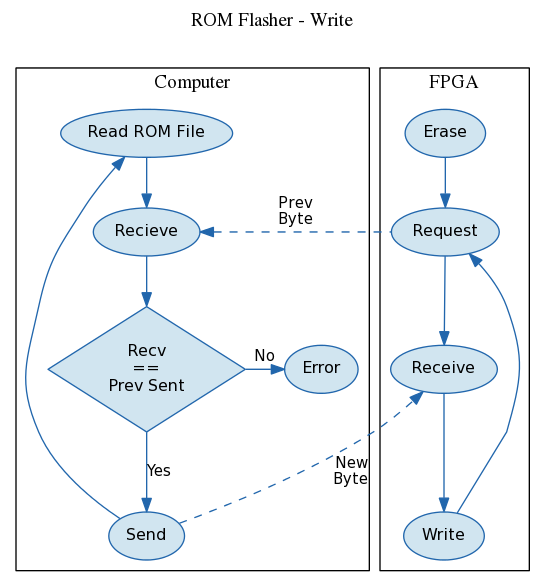
\includegraphics[height=0.65\textheight]{../../fpga/rom_flasher/doc/block_diagram_write.png}
        \column{0.5\textwidth}
            \centering Reading
            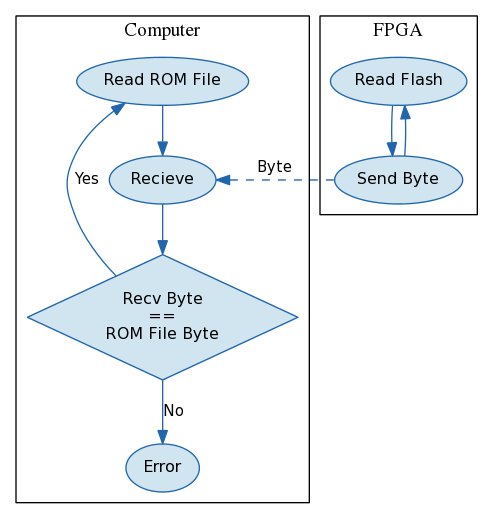
\includegraphics[height=0.65\textheight]{../../fpga/rom_flasher/doc/block_diagram_read.png}
    \end{columns}
\end{frame}


\end{document}
